\subsection{Environment}
\label{subsec:environment}

For this project, the breadboard, on which the arduino and both sensors are connected, is mounted on a swivel plate.
This allows the for easy and smooth rotation.
The board should be mounted in a way that puts the ultrasound sensor close to its center of rotation.

To create the types of junctions that have to be classified, I created two L shaped pieces, consisting of two planks of wood each, joined in a $90\deg$ angle.
Those two are sufficient to create every relevant type of environment.

% TODO: include pictures of expected data and setup
\begin{figure}
    \centering
    \includegraphics[width=0.5\linewidth]{figures/IMG_9970.jpg}
    \caption{Image of the mounted board}

    \label{fig:setup}
\end{figure}


\begin{figure}
    \centering
    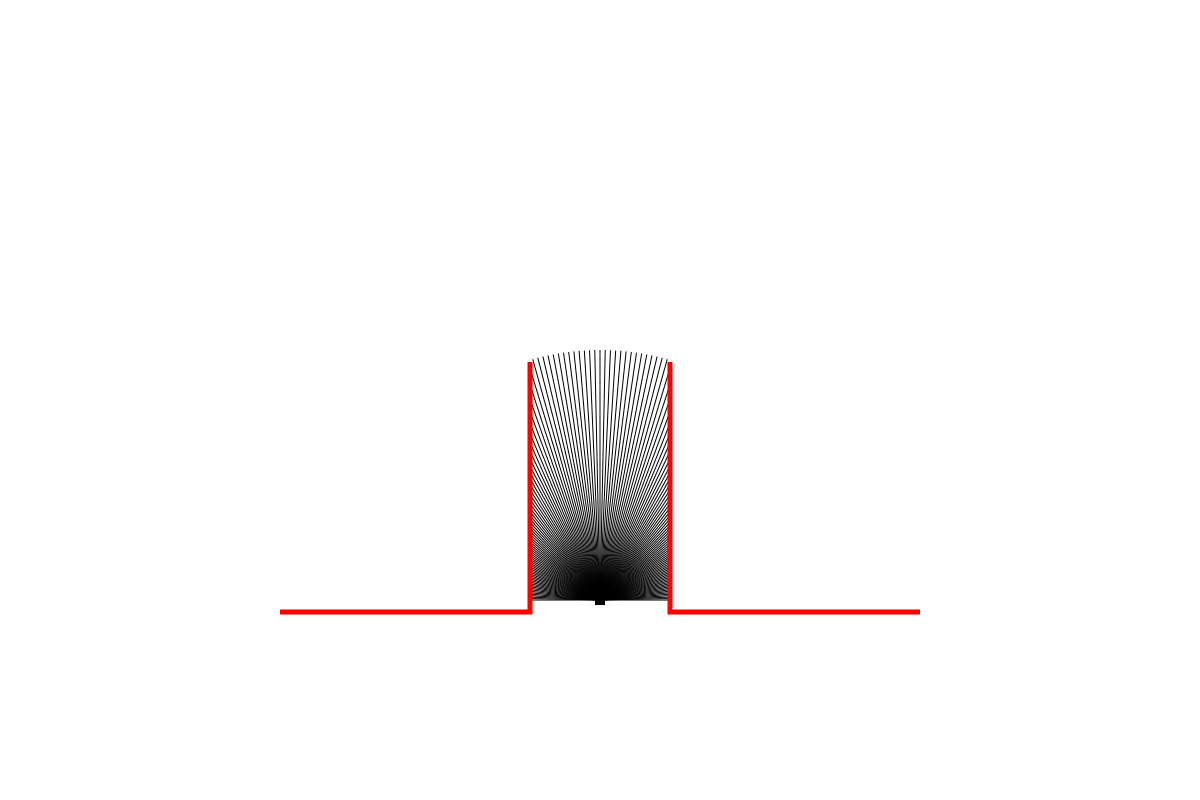
\includegraphics[width=0.3\linewidth]{figures/c.svg}
    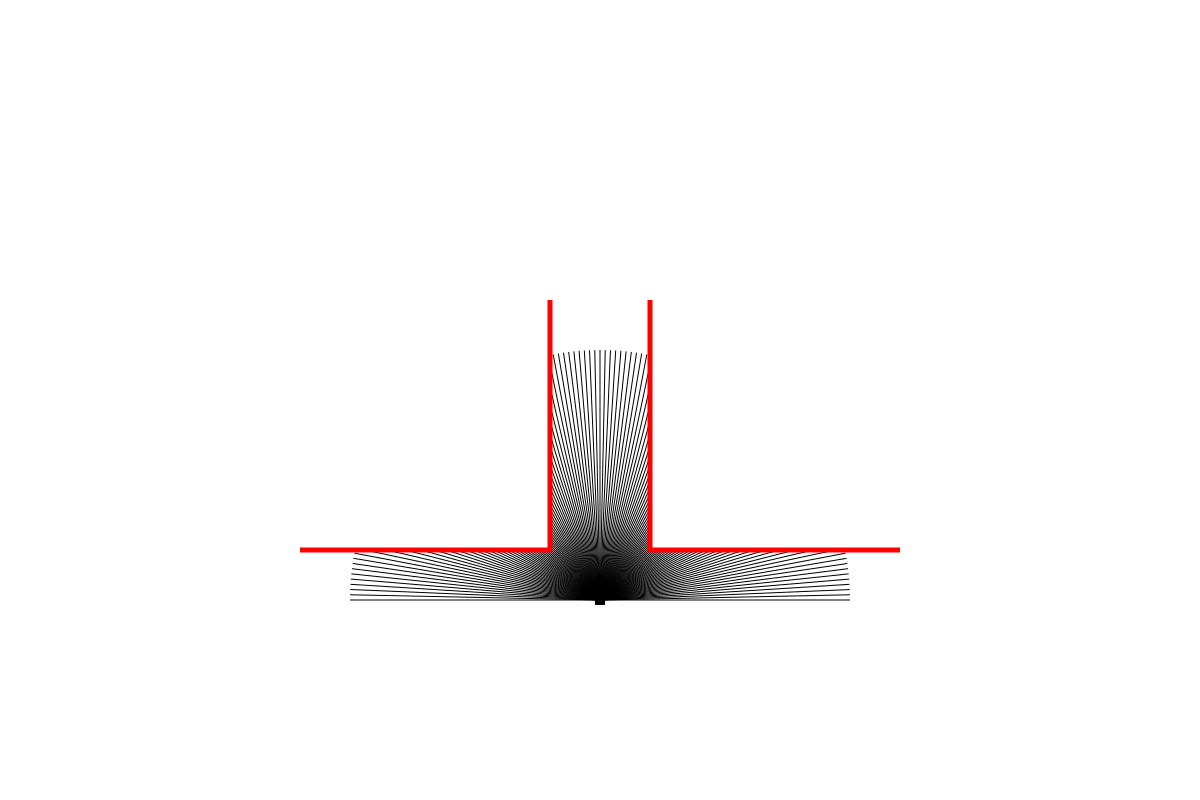
\includegraphics[width=0.3\linewidth]{figures/x.svg}
    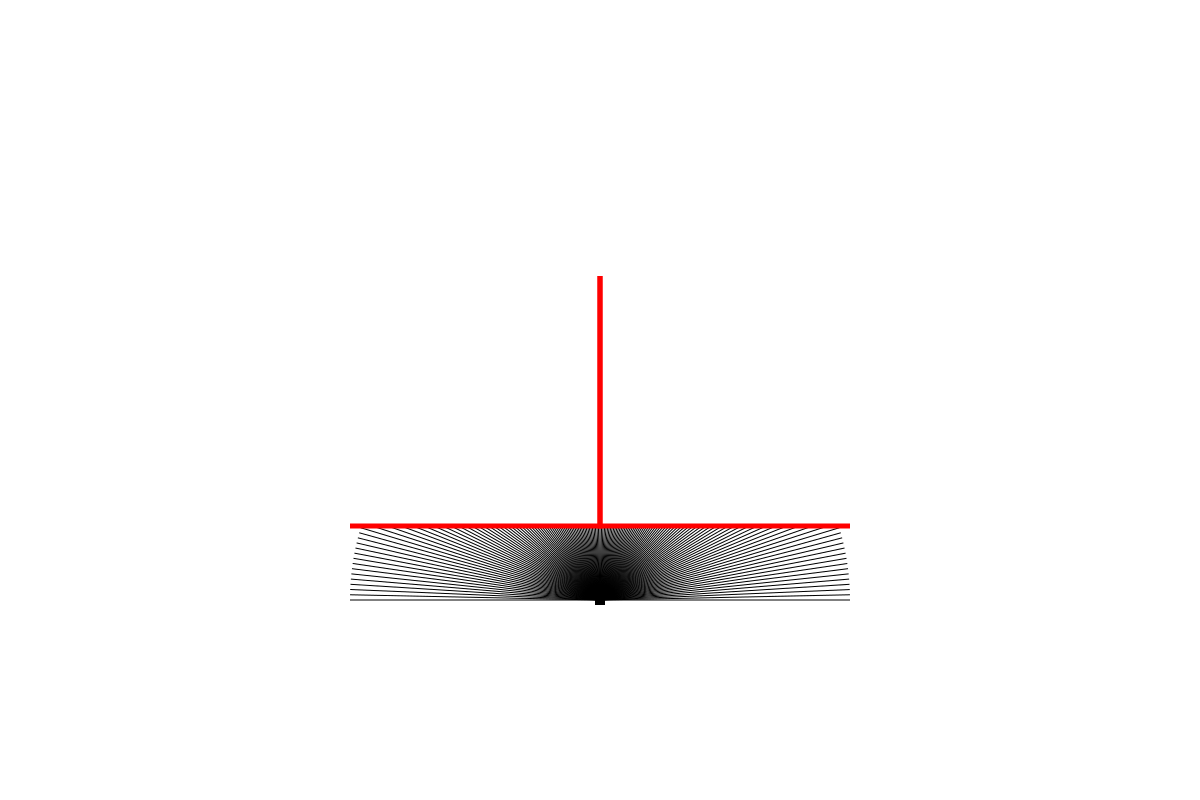
\includegraphics[width=0.3\linewidth]{figures/t.svg}
    % TODO; convert to pdf

    \caption{Image of the mounted board}

    \label{fig:env}
\end{figure}